% Beamer Presentation and Lecture Note Template
% Version 0.1
% by Paul Vesey

%%%%%%%%%%%%%%%%%%%%%%%%%%%%%%%%%%%%%
% Switch between these for presentation
% and A4 Lecture Notes
%\documentclass[ignorenonframetext,red]{beamer}     % use this for presentations and slide handouts
%\documentclass[ignorenonframetext]{beamer}     % use this for presentations and slide handouts
%\documentclass[a4paper]{article}     % use this to print the notes

%\documentclass{beamer}

%%%%%%%%%%%%%%%%%%%%%%%%%%%%%%%%%%%%%%%%
% Turn off all of these for A4 Notes
%
\mode<presentation> {
%\usetheme{lankton-keynote} % Seperate Download
%\usetheme{Madrid}
\usetheme{Antibes}
\setbeamercovered{invisible}
\setbeamertemplate{navigation symbols}{} 
}

%%\mode<presentation>{}



%%%%%%%%%%%%%%%%%%%%%%%%%%%%%%%%%%%%%%%%%%
%%%%%%%%%%%%%%%%%%%%%%%%%%%%%%%%%%%%%%%%%%

\usepackage{eurosym}
\usepackage{graphicx}
\usepackage{wasysym}
\usepackage{listings}
\usepackage{pxfonts}
\usepackage{verbatim}
\usepackage{color}
\usepackage{xcolor}
\usepackage{wrapfig}
\usepackage{hyperref}
\usepackage[nomain, xindy, toc, acronym]{glossaries}

%\newglossaryentry{html}
%{ name=HTML, description={Hypertext Markup Language is the backbone of webpages.  Static pages are simply served up by the webserver on request.  Dynamic pages are created and returned by the webserver on the fly.},
%}



%\newglossaryentry{css}
%{  name=CSS, description={Cascading Style Sheets are a way to apply styling to web-pages. It can be inline, or through an external file.  An external file is the best approach.},
%}




\newglossaryentry{Linux}
{
  name=Linux,
  description={is a generic term referring to the family of Unix-like
               computer operating systems that use the Linux kernel},
  plural=Linuces
}

\newglossaryentry{DOM1}
{
  name=DOM Level 1,
  description={The DOM Level 1 specification is separated into two parts: Core and HTML. The Core DOM Level 1 section provides a low-level set of fundamental interfaces that can represent any structured document, as well as defining extended interfaces for representing an XML document.}
}

\newglossaryentry{Apache}
{
  name=Apache,
  description={Open-source web server developed by the Apache Foundation.  One of the most widely used webservers on the planet.}
}

\newglossaryentry{JS}
{
  name=JavaScript,
  description={Scripting Language often included in web pages.  Requires an interpreter in the browser.}
}



\newglossaryentry{MySQL}{name=MySQL,
description={database engine by Oracle}}


\newglossaryentry{PDO}{name=PDO,
description={php Data Objects.  A lightweight database abstraction layer for php}}

\newglossaryentry{zxing}{name=ZXing,
description={pronounced Zebra Crossing, ZXing is an open-source bar-code scanner project.  ZXing can read standard bar-codes and QR codes}}

\newglossaryentry{QR}{name=QR,
description={Quick Response Code. A form of two dimensional machine readable image similar to a traditional bar code}}


\newglossaryentry{JavaScript}{name=JavaScript,
description={An interpreted computer language in widespread use in web applications}}


\newglossaryentry{php}{name=php,
description={php Hypertext Preprocessor. An interpreted computer language in widespread use on web servers}}



\newglossaryentry{Android}{name=Android,
description={A Linux based operating system for Smartphones and tablet computers}}



\newglossaryentry{ProGuard}{name=ProGuard,
description={A tool for optimizing and obfuscating compiled Android Apps}}

\newacronym{lvm}{LVM}{Logical Volume Manager}
\newacronym{html}{HTML}{Hypertext Markup Language}
\newacronym{xml}{XML}{Extensible Markup Language}
\newacronym{css}{CSS}{Cascading Style Sheets}
\newacronym{dom}{DOM}{Document Object Model}
\newacronym{url}{URL}{Uniform Resource Locator}
\newacronym{SQL}{SQL}{Structured Query Language}
\newacronym{oop}{OOP}{Object Orientated Programming}
\newacronym{RFID}{RFID}{Radio Frequency Identification}
\newacronym{VLE}{VLE}{Virtual Learning Environment}
\newacronym{api}{API}{Application Program Interface}
\newacronym{https}{HTTPS}{Hypertext Transfer Protocol Secure}
\newacronym{tcpip}{TCP/IP}{Transmission Control Protocol / Internet Protocol}
\newacronym{uml}{UML}{Unified Modeling Language}
\newacronym{lamp}{LAMP}{Linux, Apache, MySQL, php}
\newacronym{AMP}{LAMP}{Linux, Apache, MySQL, php}
\newacronym{ftp}{FTP}{File Transfer Protocol}
\newacronym{sdk}{SDK}{Software Development Kit}
\newacronym{lcd}{LCD}{Liquid Crystal Display}
\newacronym{ajax}{AJAX}{Asynchronous Javascript and XML}
\newacronym{IDE}{IDE}{Integrated Development Environment}
\newacronym{IE}{IE}{Microsoft Internet Explorer}
\newacronym{WiFi}{WiFi}{Wireless Local Area Network}

\makeglossaries{}
\usepackage[xindy]{imakeidx}
\makeindex




%%%%%%%%%%%%%%%%%%%%%%%%%%%%%%%%%%%%%%%%%%%%%%%%%%%%%%
%%%%%%%%%%%%%%%%%%%%%%%%%%%%%%%%%%%%%%%%%%%%%%%%%%%%%%
%
%THIS IS FOR PRINTING SLIDE HANDOUTS
%\usepackage{pgfpages}
%\pgfpagesuselayout{2 on 1}[a4paper,border shrink=5mm]

%%%%%%%%%%%%%%%%%%%%%%%%%%%%%%%%%%%%%%%%%%%%%%%%%%%%%%%
%%%%%%%%%%%%%%%%%%%%%%%%%%%%%%%%%%%%%%%%%%%%%%%%%%%%%%
%
%THIS IS FOR PRINTING A4 NOTES
%
%\usepackage{beamerarticle}    % Turn this on for A4 notes

%%%%%%%%%%%%%%%%%%%%%%%%%%%%%%%%%%%%%%%%%%%%%%%%%%%%%%

%\renewcommand\verbatim@font{\color{red}\normalfont\ttfamily}




%\usepackage{bm} 
% For typesetting bold math (not \mathbold)
%\logo{\includegraphics[height=0.6cm]{yourlogo.eps}}
%
\title[3D Studio Max (Design)]{3D Studio Max (Design)}
%
\author{Paul Vesey}
\institute[LIT]
{
Limerick Institute of Technology \\
\medskip
{\emph{paul.vesey@lit.ie}}
}
\date{2015-2016}
% \today will show current date. 
% Alternatively, you can specify a date.

\begin{document}
%

%\lstset{language=C++, frame=single}

\lstset{language=HTML,
				basicstyle=\small,
				breaklines=true,
        numbers=left,
        numberstyle=\tiny,
        showstringspaces=false,
        aboveskip=-20pt,
        frame=leftline
        }



\tableofcontents
\newpage



\begin{frame}
\titlepage
\end{frame}\begin{center}\line(1,0){250}\end{center}
%
%


\section{Introduction}




\begin{frame}
\frametitle{About me}
\begin{itemize}
	\item Paul Vesey
	\item 13B09
	\item email is best
\end{itemize}

\end{frame}
\begin{center}\line(1,0){250}\end{center}







\section{Unity3D}



\begin{frame}
\frametitle{Unity3D}
\begin{itemize}
	\item Unity is one of many Game Engines
	\item It is not the most sophisticated
	\item We will need to develop our vocabulary to effectively learn this (and other) visualization tools
\end{itemize}
\end{frame}
\begin{center}\line(1,0){250}\end{center}



\begin{frame}
       \begin{columns}
          \column{0.38\linewidth}
             \centering
						
						\begin{figure}
							\centering
								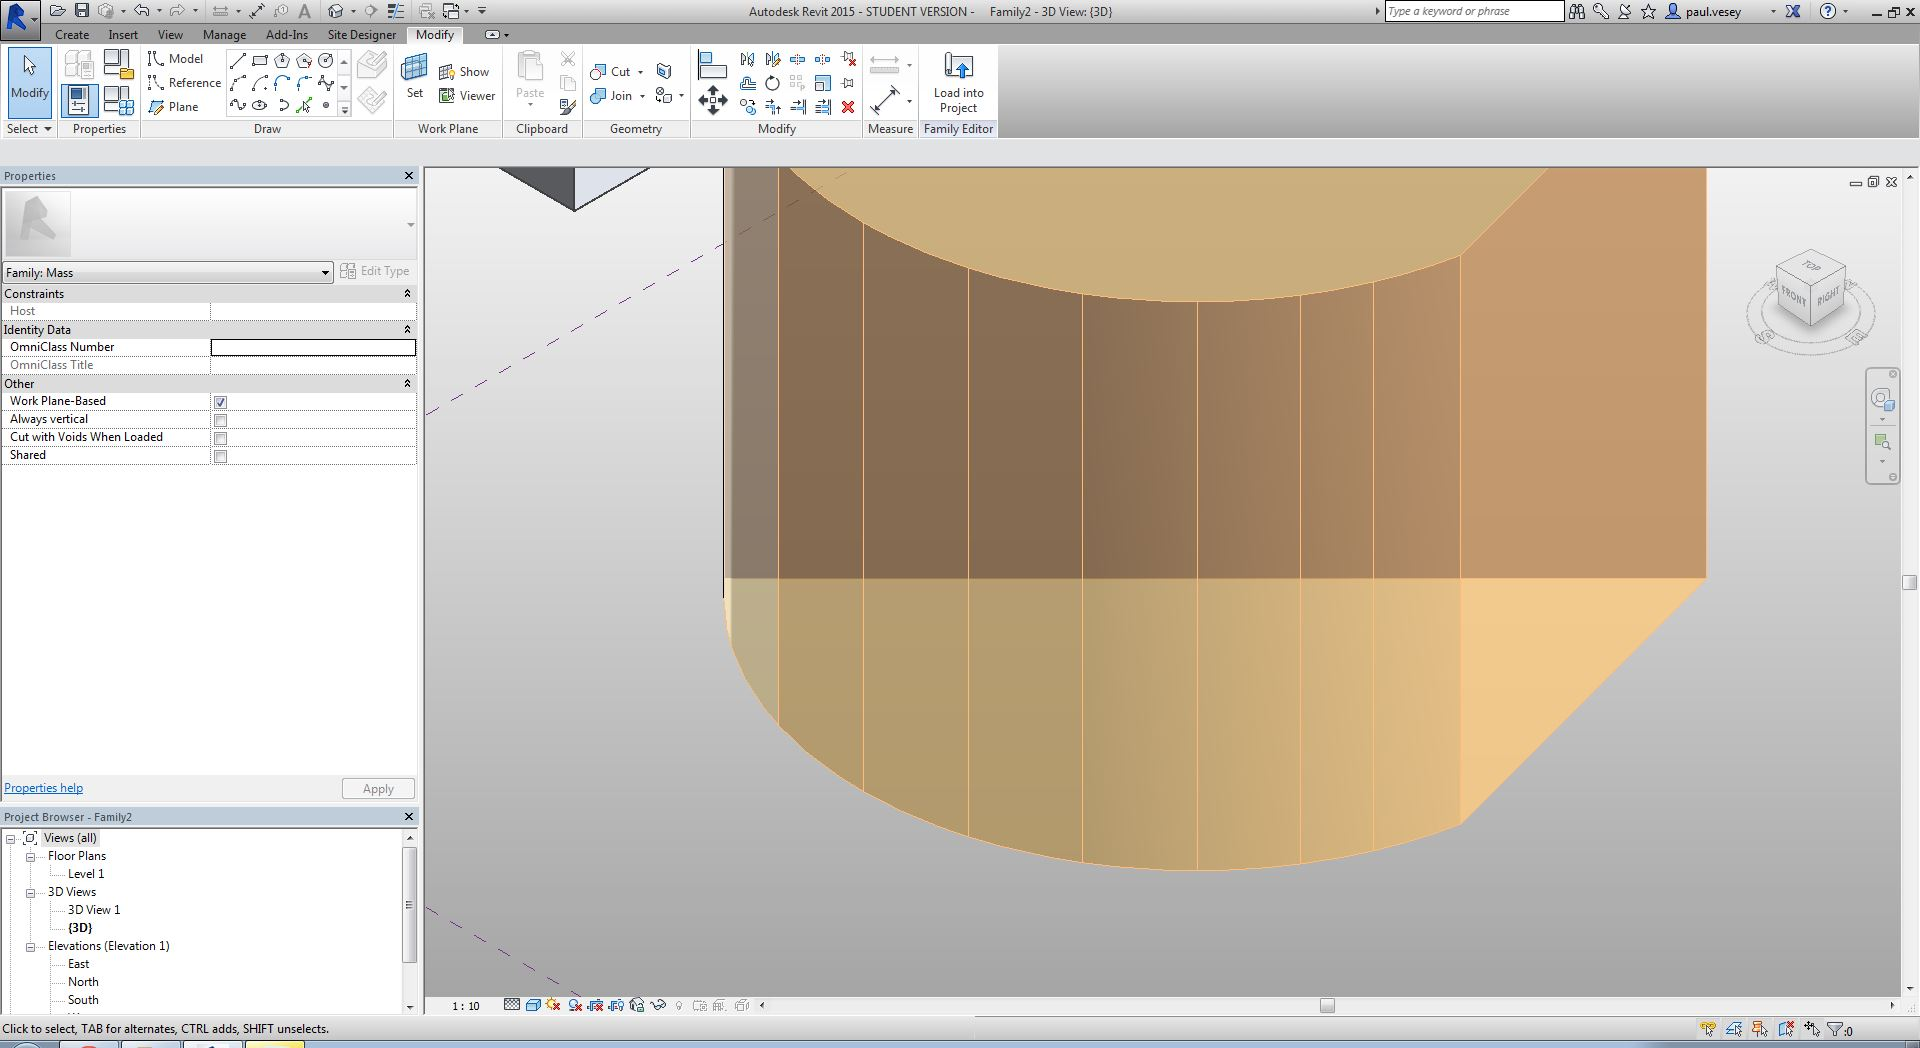
\includegraphics[height=5cm, width=3.5cm]{img/AddingEdges.JPG}
							\label{fig:AddingEdges}
						\end{figure}
						
          \column{0.58\linewidth}
              \textbf{William George Horner} (geboren in 1786, gestorven in 1837) was een Brits
                wiskundige. Hij studeerde aan de Kingswood School in Bristol, waar hij reeds op
                14(!)-jarige leeftijd een masteropleiding volgde. Daarna trok hij richting Bath
                 waar hij een school stichtte.
         \end{columns} 
\end{frame}



\section{Modeling Basics}


\subsection{Make a Chest of Drawers}

\subsection{Design Study - Create a Coffee Cup}



\section{Rendering}



\section{Cameras}

\begin{frame}
\frametitle{Lens Basics}
       \begin{columns}
          \column{0.38\linewidth}
             \centering
						
						\begin{figure}
							\centering
								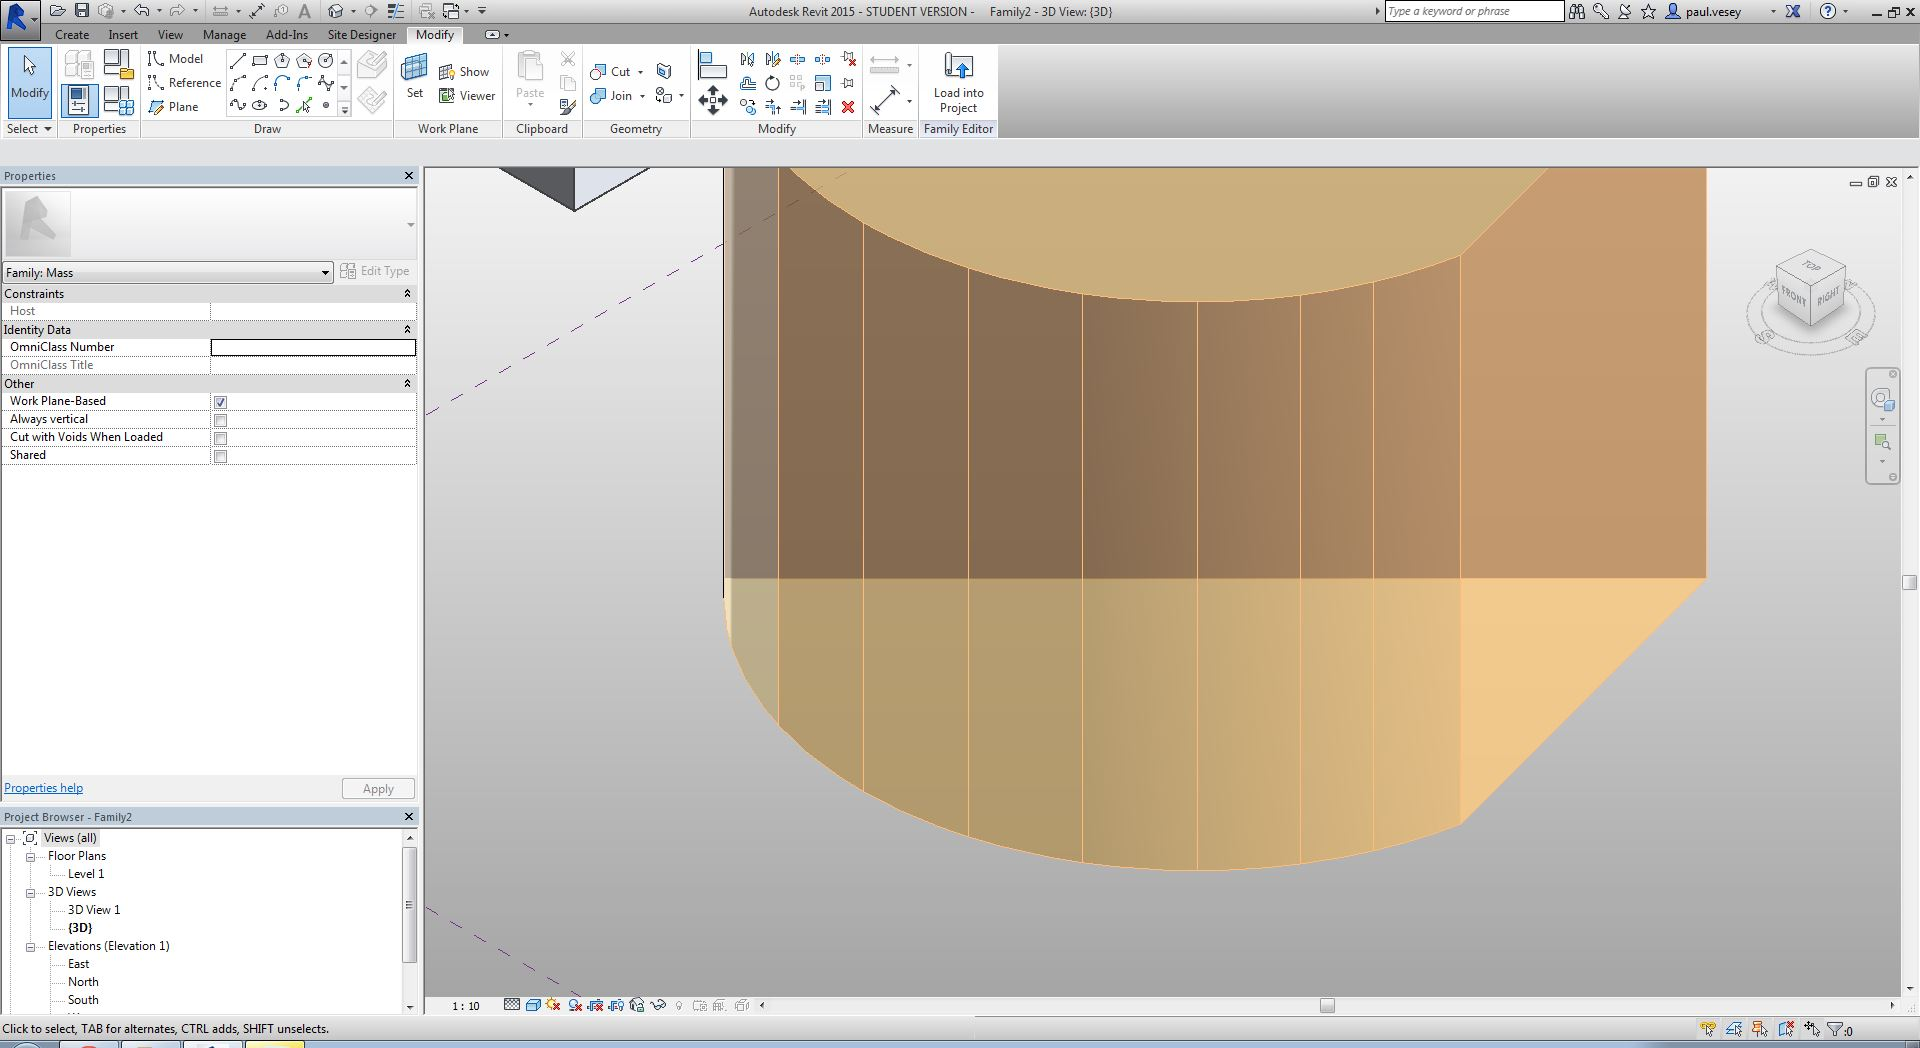
\includegraphics[height=5cm, width=3.5cm]{img/AddingEdges.JPG}
							\label{fig:AddingEdges}
						\end{figure}
						
          \column{0.58\linewidth}
						\begin{itemize}
							\item Focal Length
							\item Aperture (f-stop)
						\end{itemize}
         \end{columns} 
\end{frame}

\begin{frame}
\frametitle{Lens Basics - Aperture}
       \begin{columns}
          \column{0.38\linewidth}
             \centering
						
						\begin{figure}
							\centering
								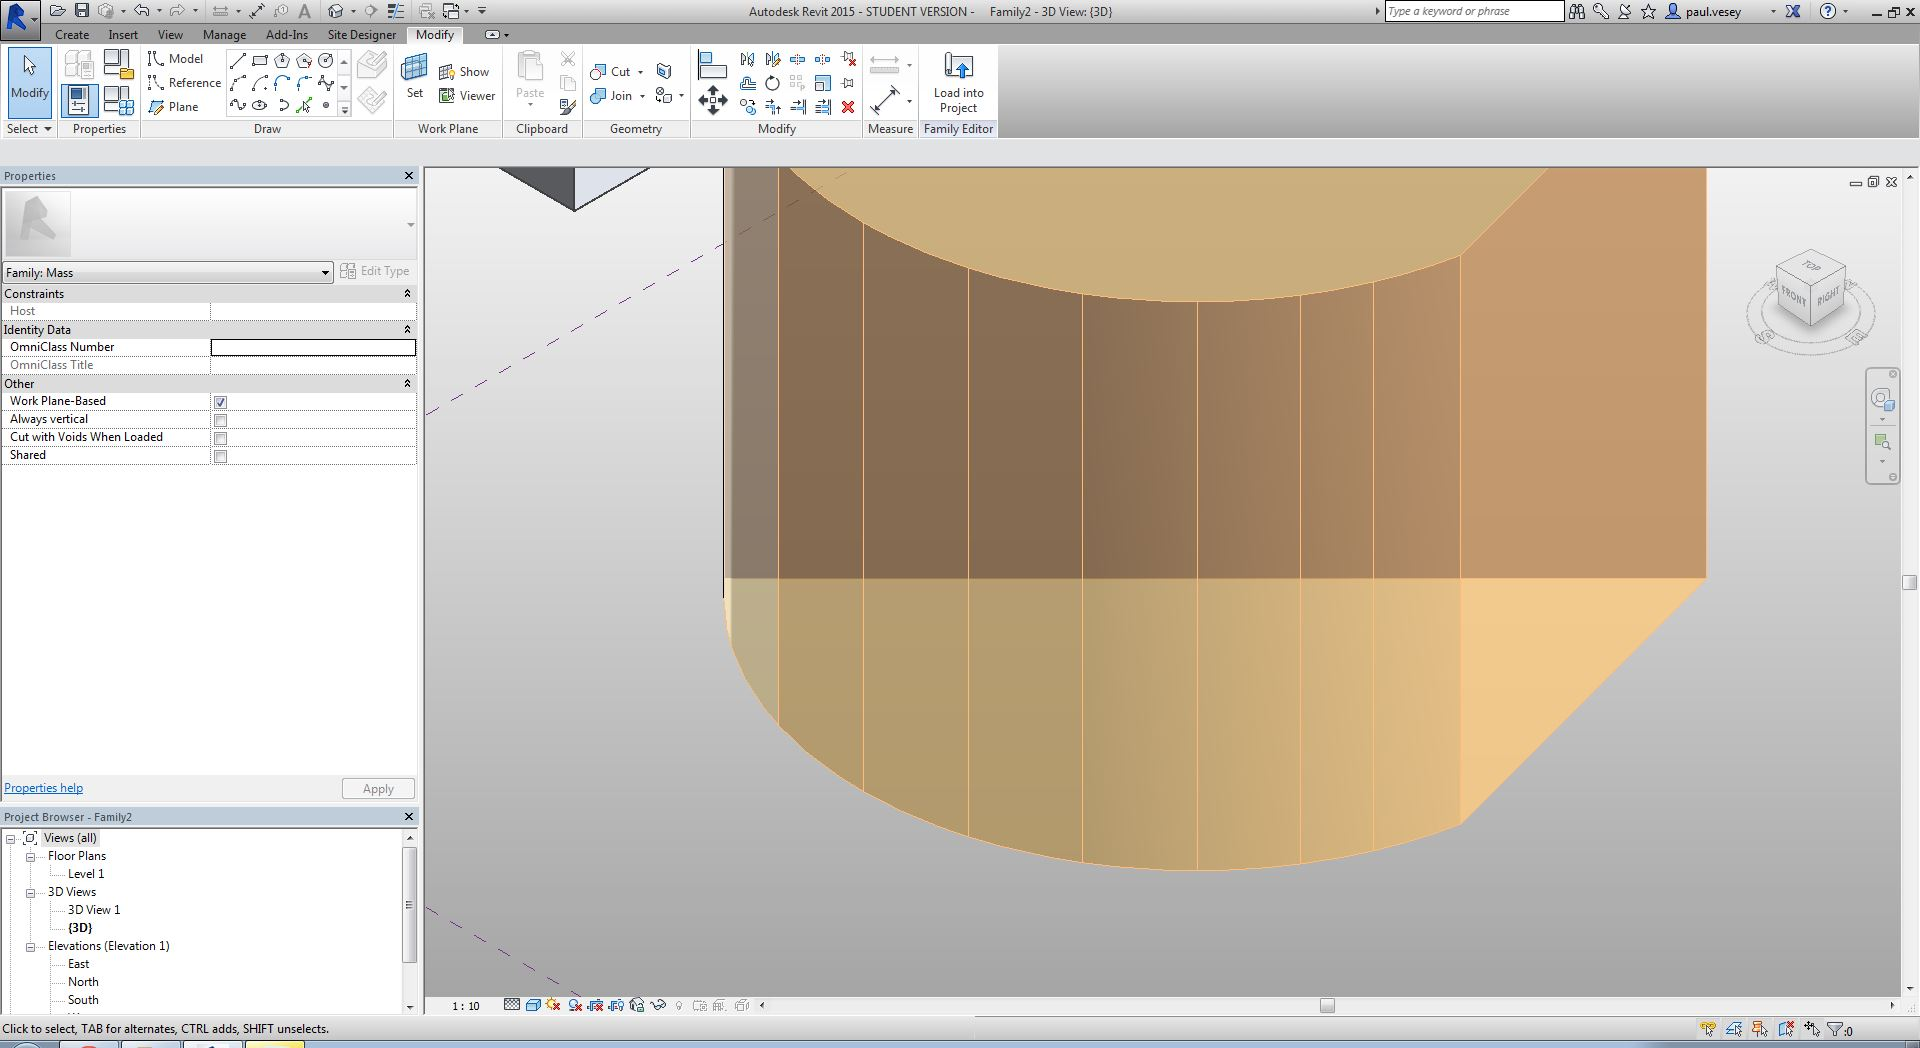
\includegraphics[height=5cm, width=3.5cm]{img/AddingEdges.JPG}
							\label{fig:AddingEdges}
						\end{figure}
						
          \column{0.58\linewidth}
						\begin{itemize}
							\item The larger the number the smaller the aperture so F22 is smaller than F1.4
							\item The larger the aperture the shorter the depth of field; so F1.4 will have a very short depth of field, compared to F22 which will keep the entire image in focus
						\end{itemize}
         \end{columns} 
\end{frame}


\begin{frame}
\frametitle{Lens Basics - Focal Length}
       \begin{columns}
          \column{0.38\linewidth}
             \centering
						
						\begin{figure}
							\centering
								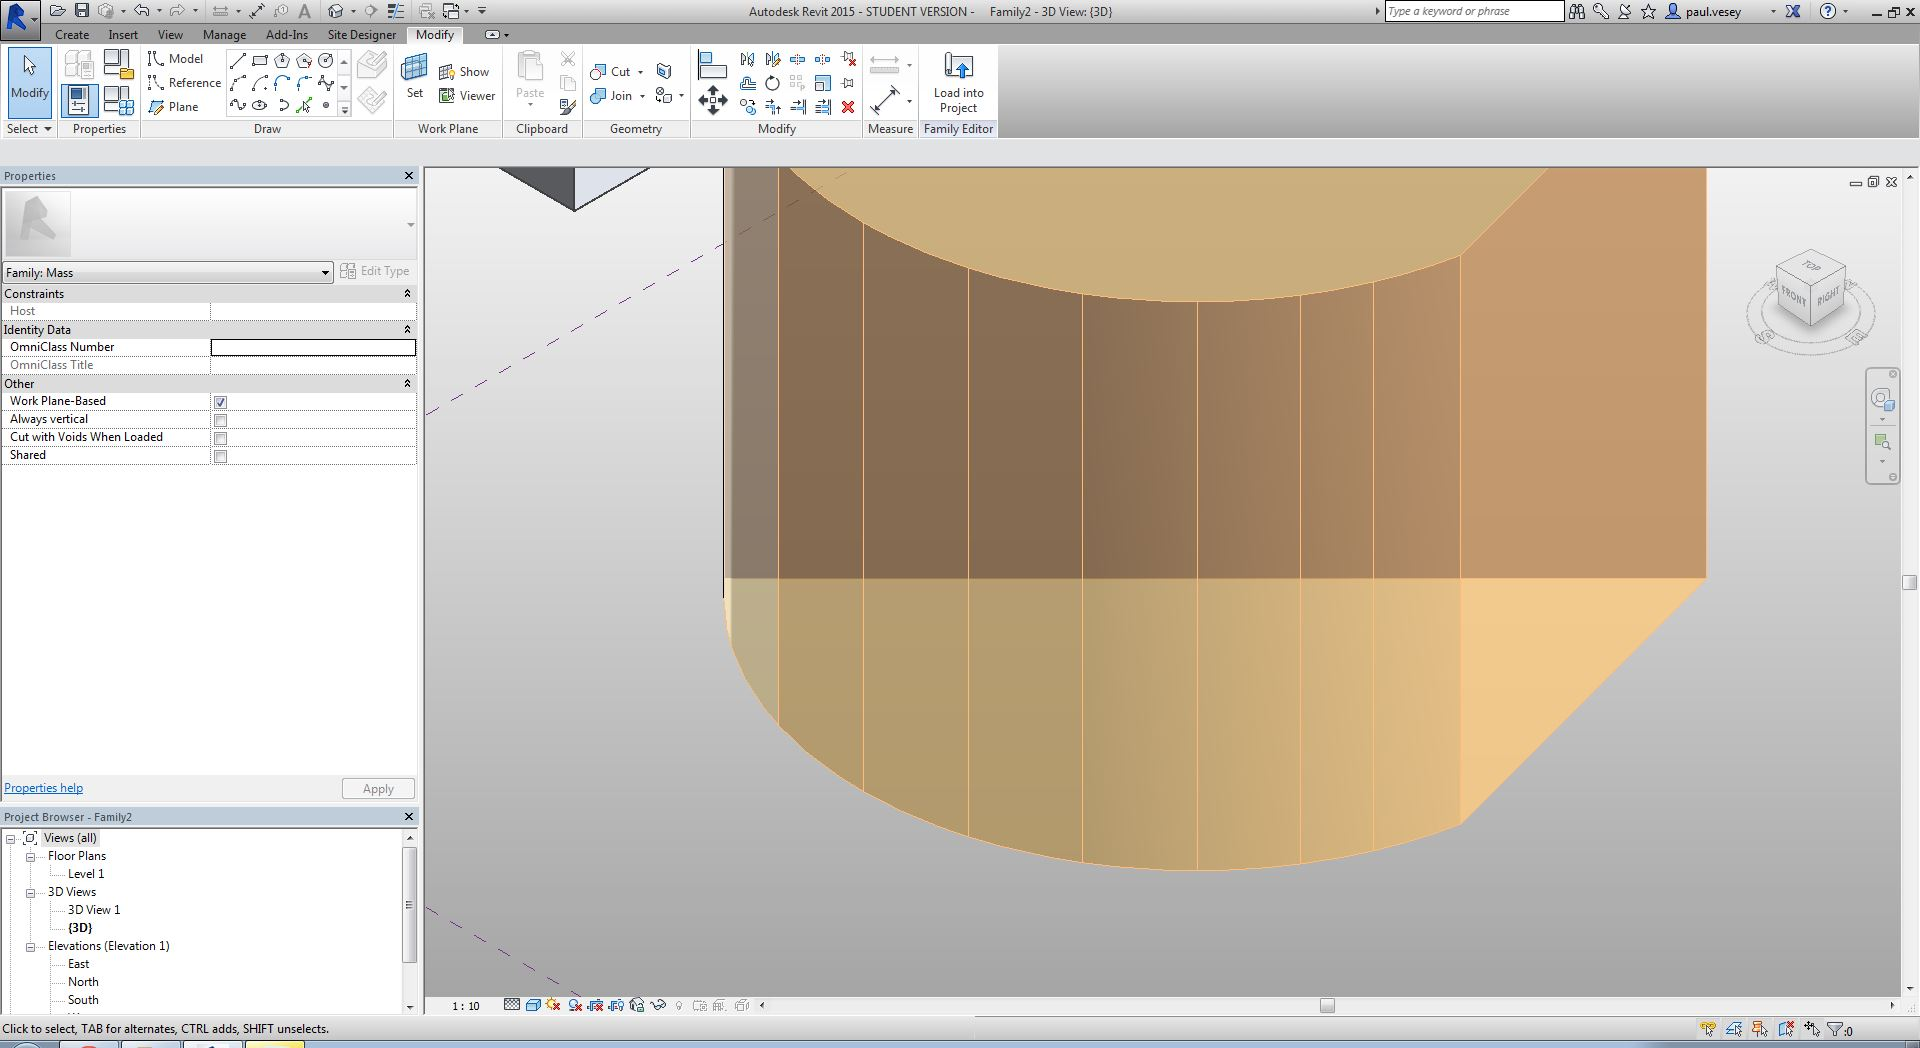
\includegraphics[height=5cm, width=3.5cm]{img/AddingEdges.JPG}
							\label{fig:AddingEdges}
						\end{figure}
						
          \column{0.58\linewidth}
						\begin{itemize}
							\item The human eye has a focal length of about 45mm.  
							\item The term 'Long Lens' typically refers to lenses over 150mm.  Wildlife photographers will often use 500mm+ lenses in order to stay back from the subject.  The trade-off is in the size of the background captured.
							\item Short lenses (such as fish-eye) are of the order of 15mm.  These may also be referred to as wide lenses.   They are often used to capture building interiors.  There can be significant levels of distortion as a result.  Smart-phones use fish-eye lenses with correction software to capture images that look more realistic
						\end{itemize}
         \end{columns} 
\end{frame}


\begin{frame}
\frametitle{Lens Basics - Mental Ray}
       \begin{columns}
          \column{0.38\linewidth}
             \centering
						
						\begin{figure}
							\centering
								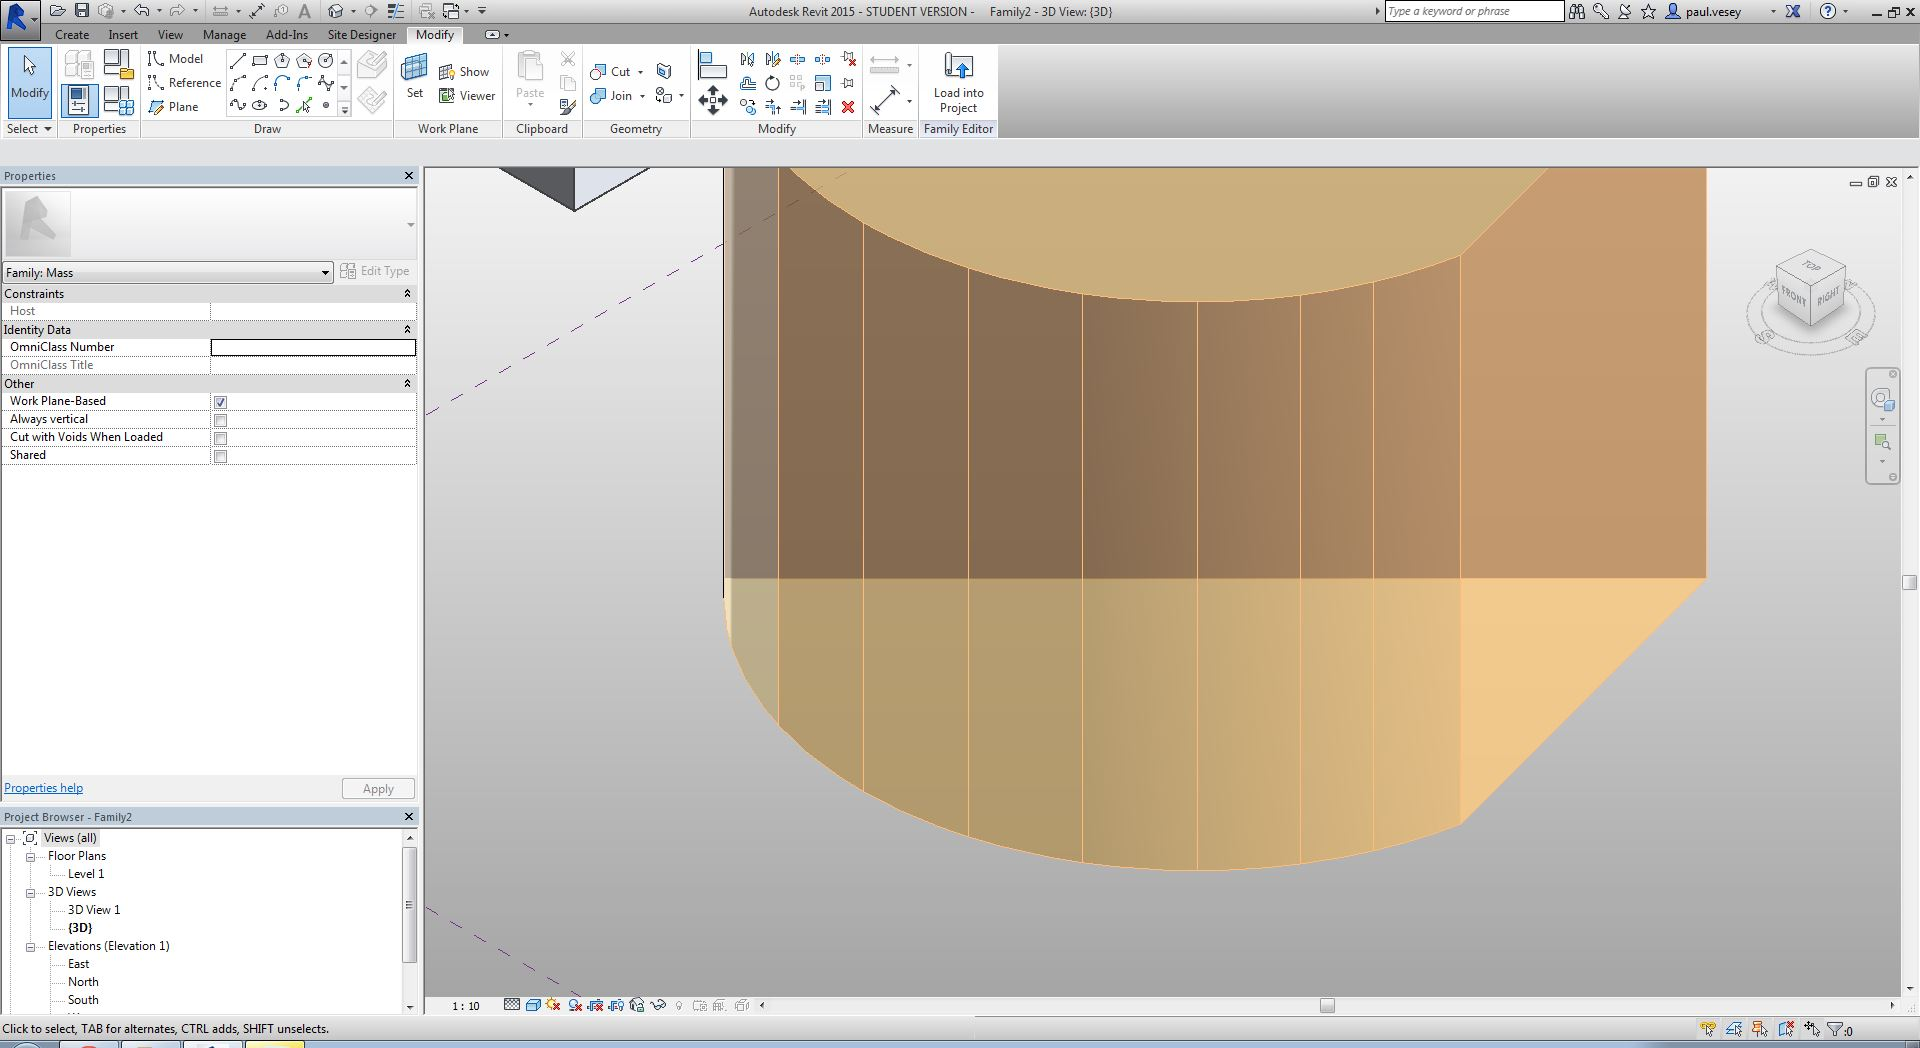
\includegraphics[height=5cm, width=3.5cm]{img/AddingEdges.JPG}
							\label{fig:AddingEdges}
						\end{figure}
						
          \column{0.58\linewidth}
						\begin{itemize}
							\item Mental Ray allows us to set both the focal length and the aperture values.  These are set in the Render Setup.  
							\item Remember to turn on 'Multi-Pass Effect'
						\end{itemize}
         \end{columns} 
\end{frame}



\subsection{Design Study - Depth of Field}


\subsection{Design Study - Focal Length}

\section{Materials}

Diffuse
Ambient
Specular (Highlights)

Normal or Bump-maps


Shaders
Blin etc.





\section{Lighting}















\section{Practicals and Assignments}



\section{3D Studio}




Editable mesh should not be used anymore.  Use Editable Poly..






\newpage

%
%This is some text 

to include chamfers
recesses
legs
union and subtraction




\subsection{Render Scene with Depth of Field x3 Renders}
Mental Ray Render with Depth of Field selected..



\bibliographystyle{plainnat}
%\bibliographystyle{Classes/CUEDbiblio}
%\bibliographystyle{Classes/jmb}
%\bibliographystyle{Classes/jmb} % bibliography style
\nocite{*}
%\renewcommand{\bibname}{Bibliography} % changes default name References to Bibliography
\addcontentsline{toc}{chapter}{Bibliography}

\bibliography{refs/references} % References file

\newpage

\printindex
\newpage





\end{document}
